\documentclass{beamer}

\usepackage{amssymb}
\usepackage{mathtools}

\title{Sommerfeld enhancement of dark matter signals at telescopes}
\author{Supervisor: Dr. Filippo Sala, Submitted by: Luca Zoppetti}
\institute{Alma Mater Studiorum - University of Bologna}
\date{22/07/2025}

\beamerdefaultoverlayspecification{<+->}

\graphicspath{ {../tex/images}, {../notebooks} }

\begin{document}

\frame{\titlepage}

\begin{frame}
\frametitle{Structure of the talk}
\begin{itemize}
	\item Dark matter evidence
	\item Indirect detection and Sommerfeld enhancement
	\item Quick mathematical review
	\item Results and conclusions
\end{itemize}
\end{frame}

\begin{frame}
\frametitle{Dark matter evidence (1): galaxy clusters}
In 1933, Fritz Zwicky estimated the velocity dispersion in the Coma cluster:
\[
	\sqrt{\langle v^2 \rangle } \simeq 80 \mathrm{km / s}
\]
\pause
The measured velocity dispersion along the line of sight is
\[
	v_{los} \sim 10^3 \mathrm{km / s} 
\]
\pause
Something doesn't add up!
\end{frame}

\begin{frame}
\frametitle{Dark matter evidence (1): galaxy clusters}
Use the virial theorem to estimate the mass in the cluster from known observational data:
\[
	\langle T \rangle = - \frac{1}{2} \langle U \rangle 
\]
\pause
% Known observational data:
% \begin{itemize}[<*>]
% 	\item \(v_{los} \sim 10^3 \mathrm{km / s} \)
% 	\item Distance is \(d \sim 100 \mathrm{Mpc} \)
% 	\item Angular radius is \(\theta \sim 1^{\circ } \)
% 	\item It is approximately spherically symmetric
% \end{itemize}
% \pause
We get
\[
	M \simeq 2 \times 10^{15} M_\odot
\]
\pause
It's off by one order of magnitude compared to the visible mass of \(10^{14} M_\odot\)!
\end{frame}

\begin{frame}
\frametitle{Dark matter evidence (2): galactic rotation curves}
From Newtonian mechanics, we expect
\[
	v(r) = \sqrt{\frac{GM(r)}{r}} 
\]
\pause
Observations by Rubin and Ford (1970), Roberts and Whitehurst (1975), and Carignan et al. (2006) show that velocity curves flatten at large radii.
\end{frame}

\begin{frame}
\frametitle{Dark matter evidence (2): galactic rotation curves}
\begin{figure}[htbp]
	\centering
	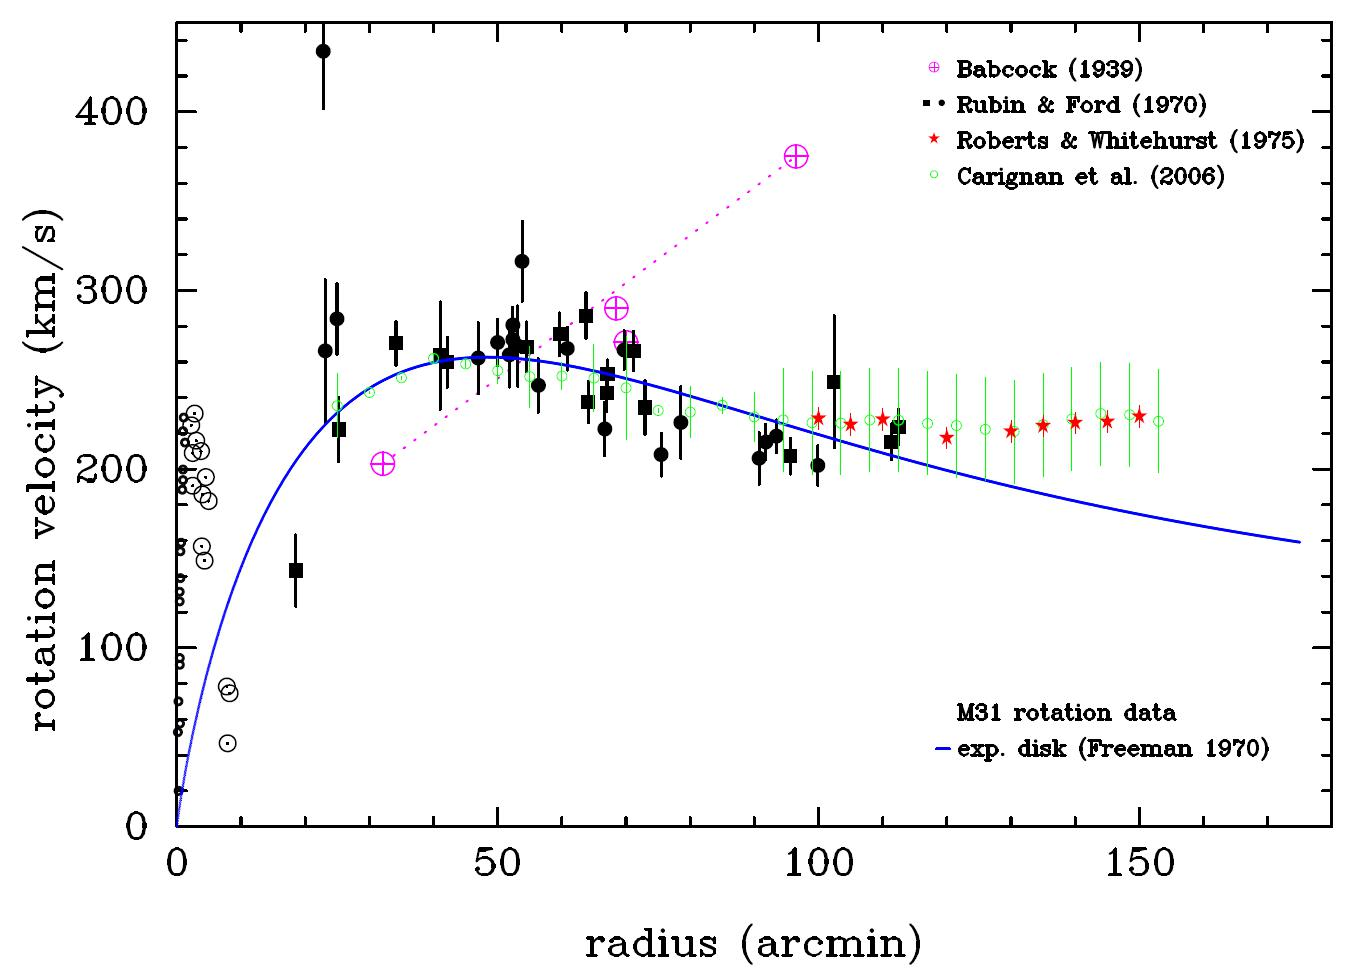
\includegraphics[width=0.8\textwidth]{rotation_curves.jpg}
	\caption{Rotational velocity data points for the M31 galaxy. In solid blue: theoretical prediction. Credits for the figure: Albert Bosma.}
	\label{fig:rotation_curves}
\end{figure}
\end{frame}

\begin{frame}
\frametitle{Dark matter evidence (2): galactic rotation curves}
The curve would flatten in the case of \(M \propto r\) at large radii. Several possible profiles exist (from simulations), NFW used in reference paper:
\[
	\rho_{\mathrm{NFW} } (r) = \frac{\rho _s}{\frac{r}{r_s} \left( 1+ \frac{r}{r_s} \right) ^2}
\]
\end{frame}

\begin{frame}
\frametitle{Dark matter evidence (3): the Bullet cluster}
\begin{figure}[htbp]
	\centering
	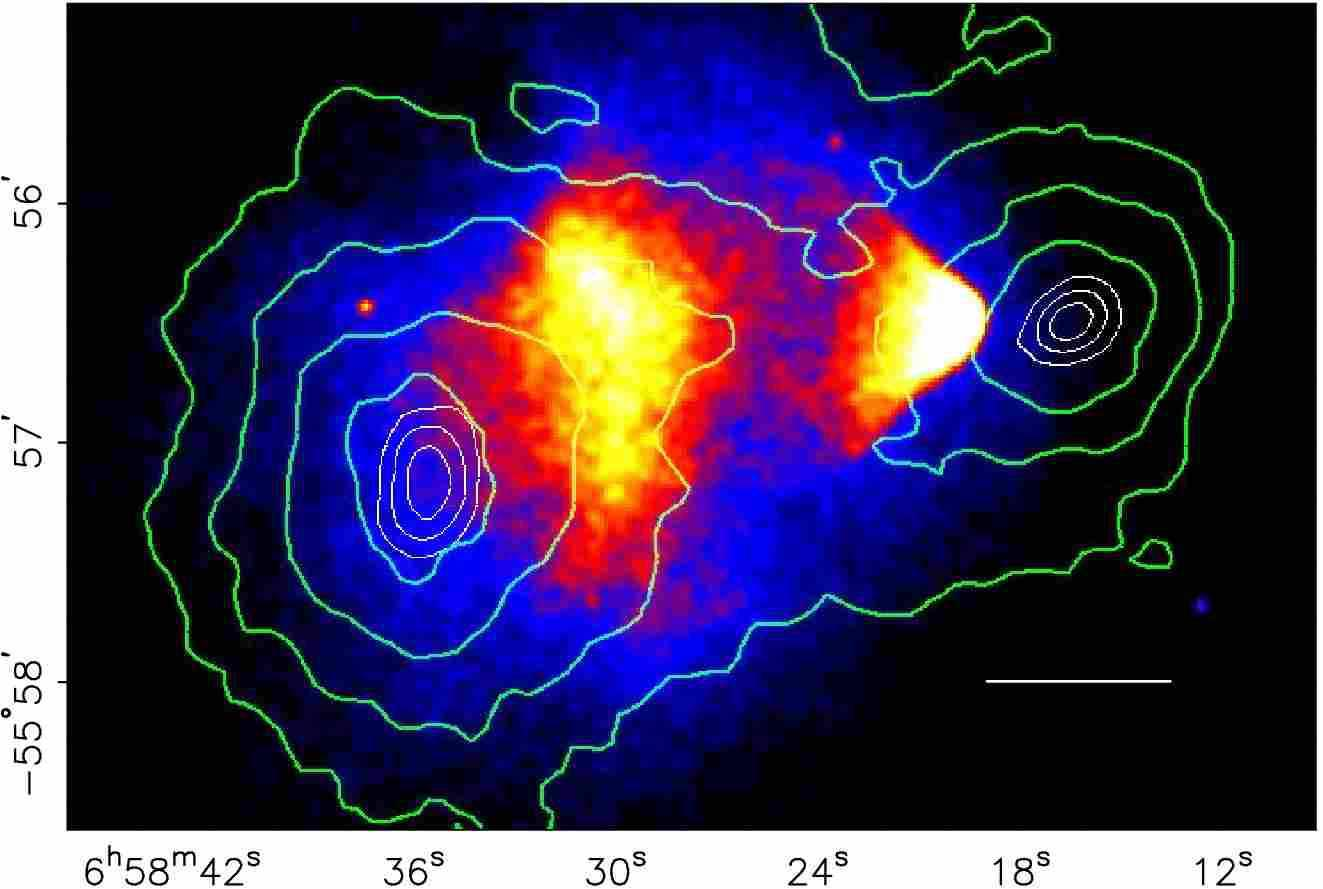
\includegraphics[width=0.8\textwidth]{bullet.jpg}
	\caption{The colormap shows X-ray-emitting matter. The green contours show the gravitational lensing signal. The two centres of mass are clearly displaced. Credits: Clowe et al. (2006).}
	\label{fig:bullet}
\end{figure}
\end{frame}

\begin{frame}
\frametitle{Dark matter evidence (4): summary}
The universe wouldn't look the way it does without dark matter:
\begin{itemize}
	\item It shaped the CMB acoustic peaks
	\item It acted as a catalyzer for large-scale structure formation (galaxies, clusters)
\end{itemize}
\pause
All of this evidence is independent and is explained at once by the hypothesis of dark matter!
\pause
To reproduce the observations, we expect dark matter to be cold, non-interacting matter with adiabatic inhomogeneities.
\end{frame}

\begin{frame}
\frametitle{Indirect detection}
\begin{itemize}
	\item We assume dark matter can annihilate or decay into standard model particles that can travel to Earth and be detected.
	\item Indirect detection refers to experiments looking for an excess of cosmic rays due to dark matter annihilation or decay.
	\item No discovery yet, but very strict bounds on the annihilation cross section.
\end{itemize}
\end{frame}

\begin{frame}
\frametitle{Indirect detection}
\begin{figure}[htbp]
	\centering
	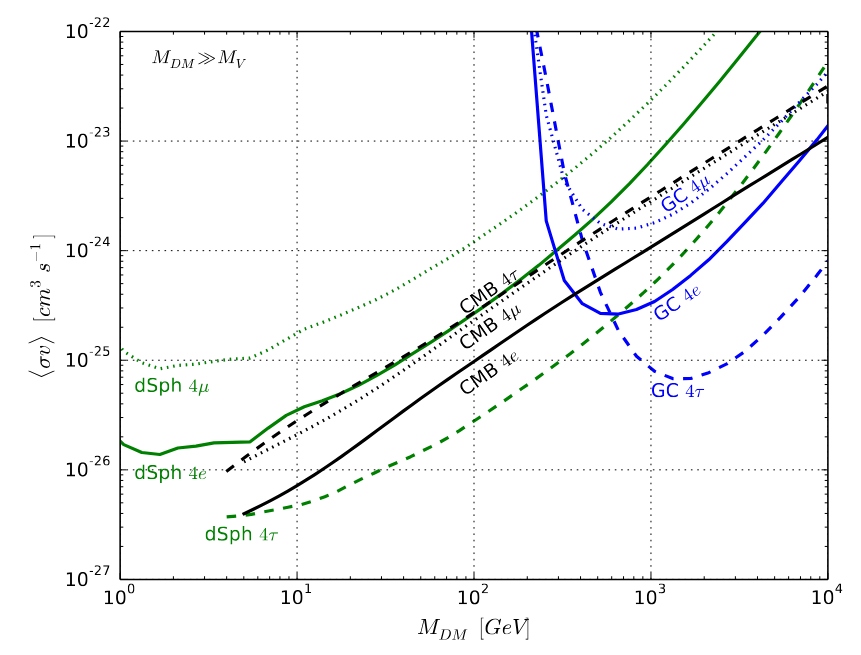
\includegraphics[width=0.75\textwidth]{fermi-data.png}
	\caption{The cross section bounds derived from Fermi-LAT (green), H.E.S.S. (blue) and CMB (black) observations presented by Profumo et al. (2018) in the reference paper for this work.}
	\label{fig:fermi}
\end{figure}
\end{frame}

\begin{frame}
\frametitle{Indirect detection}
Promising sources for indirect detection have:
\begin{itemize}
	\item High density of dark matter
	\item Proximity to us
	\item Extended across a large volume
	\item Accompanied by a low astrophysical background
\end{itemize}
\pause
Dwarf spheroidal galaxies (studied by Fermi-LAT) are particularly favorable because of the last point.
\end{frame}

\begin{frame}
\frametitle{Sommerfeld enhancement}
\begin{itemize}
	\item Assume dark matter is subject to a new "dark force" mediated by the carrier \(\phi\)
	\item Non-relativistic quantum mechanical effect: the introduction of this long-range potential affects the cross section of a process happening locally (e.g.: a point-like annihilation)
	\item Classical analogy: object falling into a star (with and without gravity)
	\item If the process is point-like, \(\sigma \propto \vert \psi(0) \vert ^2\)
\end{itemize}
\pause
The Sommerfeld enhancement factor is
\[
	S \coloneqq \frac{\sigma }{\sigma _0} = \frac{\vert \psi (0) \vert ^2 }{\vert \psi^{(0)}(0) \vert ^2 }
\]
\end{frame}

\begin{frame}
\frametitle{The Coulomb approximation}
Usually, the potential is modeled as a Yukawa potential:
\[
	V(r) = -\frac{\alpha }{r} e^{- m_{\phi } r }
\]
\pause
Here, we approximate \(m_\phi = 0\) and thus use a Coulomb-like potential:
\[
	V(r) = - \frac{\alpha }{r}
\]
\pause
The approximation is valid if the range of the force is larger than the De Broglie wavelength of the system
\[
	\frac{M_{DM} v_{rel} }{2 m_{\phi } }
\]
\end{frame}

\begin{frame}
\frametitle{Quick mathematical pointers}
\begin{itemize}
	\item The goal is to solve the Schrödinger equation with the afore-mentioned potential
	\item Reduce to one-body problem
	\item Reduce to radial problem by expanding in terms of spherical harmonics
	\item Realize that all terms vanish apart from the one with \(l=0\)
	\item Solve the one-dimensional problem by leading back to a confluent hypergeometric equation
\end{itemize}
\pause
Solution:
\[
	S = 2\pi \frac{\alpha }{v_{rel} } \frac{1}{1- e^{-2\pi \frac{\alpha }{v_{rel} }}}
\]
\end{frame}

\begin{frame}
\frametitle{Experimental implications: theoretical framework}
We are now considering the impact on the interpretation of the Fermi-LAT limits presented earlier.\\
We are considering a dark matter model where:
\begin{itemize}
	\item Dark matter is non-self-conjugate and the cross section that gives the correct dark matter relic abundance is \(\langle \sigma v \rangle_{relic} = 4.4 \times 10^{-26} \mathrm{cm ^3 s^{-1} }  \)
	\item It interacts and annihilates through a "dark interaction" mediated by \(\phi \)
	\item It decays to \(4\tau \) leptons, so that the Fermi-LAT limit in the previous figure is the strongest one
	\item \(M_{DM} \gg m_{\phi } \)
\end{itemize}
\end{frame}

\begin{frame}
\frametitle{Experimental implications: Sommerfeld enhancement}
The cross section without Sommerfeld enhancement is independent of velocity:
\end{frame}

\end{document}